% Created 2022-09-06 Tue 11:29
% Intended LaTeX compiler: pdflatex
\documentclass[presentation]{beamer}
\usepackage[utf8]{inputenc}
\usepackage[T1]{fontenc}
\usepackage{graphicx}
\usepackage{longtable}
\usepackage{wrapfig}
\usepackage{rotating}
\usepackage[normalem]{ulem}
\usepackage{amsmath}
\usepackage{amssymb}
\usepackage{capt-of}
\usepackage{hyperref}
\usepackage{color}
\usepackage{listings}
\definecolor{codepurple}{rgb}{0.58,0,0.82}
\lstset{keywordstyle=\color{magenta}, stringstyle=\color{codepurple}, showspaces=false, basicstyle=\scriptsize\ttfamily, frame=single, breaklines=true}
\usetheme{boxes}
\usecolortheme{orchid}
\author{Arunkumar M V}
\date{\today}
\title{Pulsar Search with Random Forest on FPGAs}
\hypersetup{
 pdfauthor={Arunkumar M V},
 pdftitle={Pulsar Search with Random Forest on FPGAs},
 pdfkeywords={},
 pdfsubject={},
 pdfcreator={Emacs 28.1 (Org mode 9.6)}, 
 pdflang={English}}
\begin{document}

\maketitle

\section*{Intro}
\label{sec:org837c248}
\begin{frame}[label={sec:orgc2c5c5d}]{Introduction}
This presentation outlines the implementation of random forest classifier (RFC) in hardware intended for FPGAs.
\end{frame}

\begin{frame}[label={sec:org6d904e2}]{High-level project description}
The project produces hardware designs of RFCs in the following manner:
\begin{itemize}
\item Training of the RFC is done using a python application - \emph{(Software stage)}.
\item Tree structures are then extracted and used to create verilog designs using chisel3-based parameterized circuit generators - \emph{(Hardware stage)}.
\item Generated design may then be tested using an in-house verilator-based simulator or used for synthesis using external FPGA toolchains - \emph{(Run stage)}
\end{itemize}
\end{frame}

\section*{Tech aspects}
\label{sec:orgae2416d}
\begin{frame}[label={sec:orgbea22de}]{Apporach}
The following slides present our approach. The project is divided into the following modules/stages:
\begin{itemize}
\item \emph{Software stage}
\item \emph{Hardware stage}
\item \emph{Run stage}
\end{itemize}
\end{frame}

\begin{frame}[label={sec:orgf3cc294}]{Build pipeline}
The aforementioned stages are linked together to form the \alert{build pipeline}. The stages and overall pipeline have been implemented with Scala.
\begin{center}
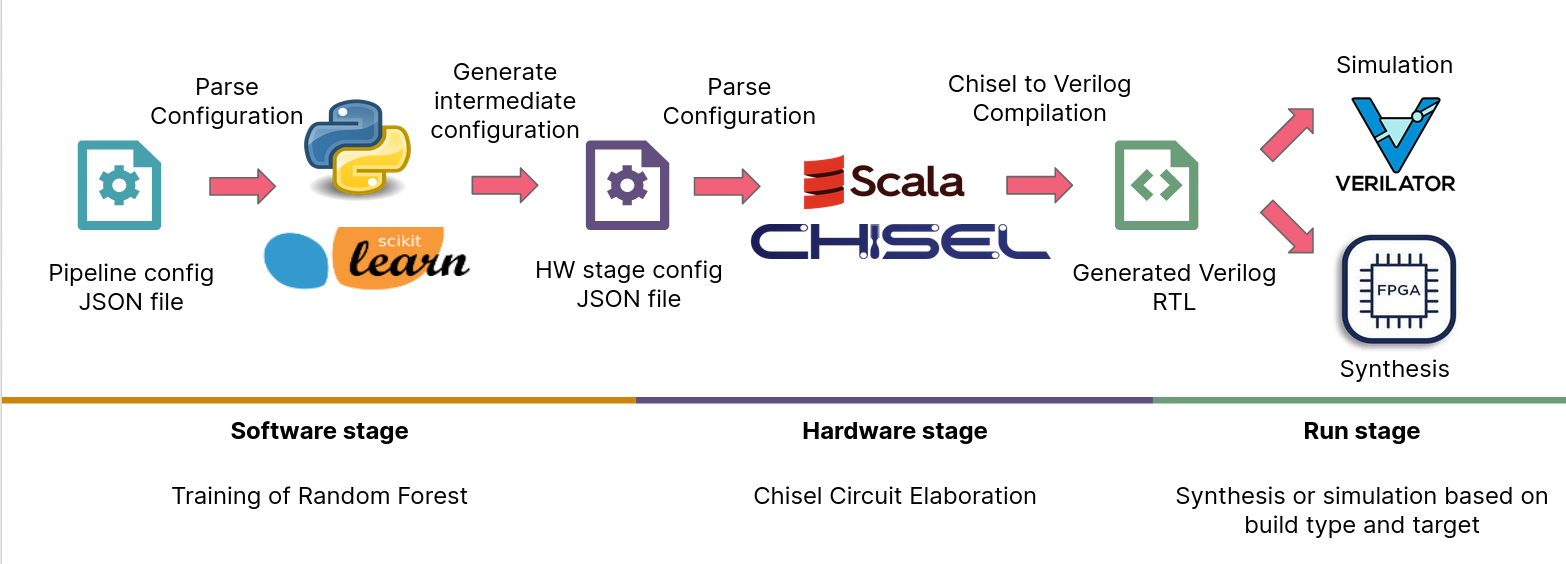
\includegraphics[width=.9\linewidth]{../images/build-pipeline.png}
\end{center}
\end{frame}

\begin{frame}[label={sec:orgf6cccd6}]{Configuring the build pipeline}
\begin{itemize}
\item A \alert{JSON-based configuration system} is used to configure the build pipeline
\item Configuration file contains various parameters to be used by the different pipeline stages
\item Enables the pipeline to be \alert{versatile and user-friendly}
\end{itemize}
\end{frame}

\begin{frame}[label={sec:org8188d05},fragile]{Example input configuration}
 \lstset{language=java,label= ,caption= ,captionpos=b,numbers=none}
\begin{lstlisting}
{
    "dataset": "datasets/HTRU_2.csv",
    "input_headers": ["Mean of the integrated profile", "Standard deviation of the integrated profile", "Excess kurtosis of the integrated profile", "Skewness of the integrated profile", "Mean of the DM-SNR curve", "Standard deviation of the DM-SNR curve", "Excess kurtosis of the DM-SNR curve", "Skewness of the DM-SNR curve"],
    "target_header": "Result",
    "train_split_size": 0.7,
    "n_estimators": 100,
    "max_leaf_nodes": 3,
    "build_type": "test",
    "build_target": "sim",
    "fixed_point_width": 32,
    "fixed_point_bp": 16,
    "opt_majority_voter": "area"
}
\end{lstlisting}
\end{frame}

\begin{frame}[label={sec:orgc49fe33}]{Build types and targets}
The build type and target determine the final products that the build pipeline generates. These are given as input configuration parameters in the JSON file.
\end{frame}

\begin{frame}[label={sec:org009e90e},fragile]{Build types}
 The build type decides which type of design is generated during the build.

\begin{block}{Possible build types}
\begin{itemize}
\item \texttt{test}
\begin{itemize}
\item Generates a ``test harness'' module that wraps around a random forest classifier module
\item This module contains the test data and expected results and automatically tests the random forest classifier module
\item This build is meant for development and verification purposes
\end{itemize}

\item \texttt{production}
\begin{itemize}
\item Generates a random forest classifier module with appropriate communication support
\item This build is meant for deploying to production
\end{itemize}
\end{itemize}

\alert{NOTE: Currently only test builds are supported. Support for production builds will be added in the future}
\end{block}
\end{frame}

\begin{frame}[label={sec:orgd2ea943},fragile]{Build targets}
 The build target decides what is done with the generated verilog design during the build.

\begin{block}{Possible build targets}
\begin{itemize}
\item \texttt{simulation}
\begin{itemize}
\item May be used to simulate the generated verilog design
\item Builds a verilator-based simulator model and runs the simulator to verify the behaviour of the module
\end{itemize}

\item \texttt{synthesis}
\begin{itemize}
\item May be used when the generated modules are to be synthesised by an external FPGA tool chain
\item Basically causes the build pipeline to exit after verilog generation from chisel
\end{itemize}
\end{itemize}
\end{block}
\end{frame}

\begin{frame}[label={sec:org07acb6f}]{Software stage}
The software stage performs the training of the RFC. It performs the following steps:

\begin{enumerate}
\item Checks for / creates a python virtual environment
\item Installs the required python libraries
\item Reads the input pipeline configuration JSON file
\item Loads and splits the dataset into training and testing data
\item Performs the fitting/training of the random forest classifier
\item Outputs the decision trees data structures and other configurations to the hardware stage as a JSON file
\end{enumerate}
\end{frame}

\begin{frame}[label={sec:org5a8b9c0}]{Hardware stage}
The hardware stage generates the verilog design based on input configuration. It performs the following steps:

\begin{enumerate}
\item Reads the configuration JSON file generated by the software stage
\item Supplies the required chisel generator module with necessary parameters
\item Performs the circuit elaboration/compilation
\item Outputs the run stage configuration as an intermediate Scala object
\end{enumerate}
\end{frame}

\begin{frame}[label={sec:org6c43e30}]{Hardware architecture}
The figure below depicts the overall architecture of the RFC implemented in Chisel. The following slides delve into different modules present in this architecture.
\begin{center}
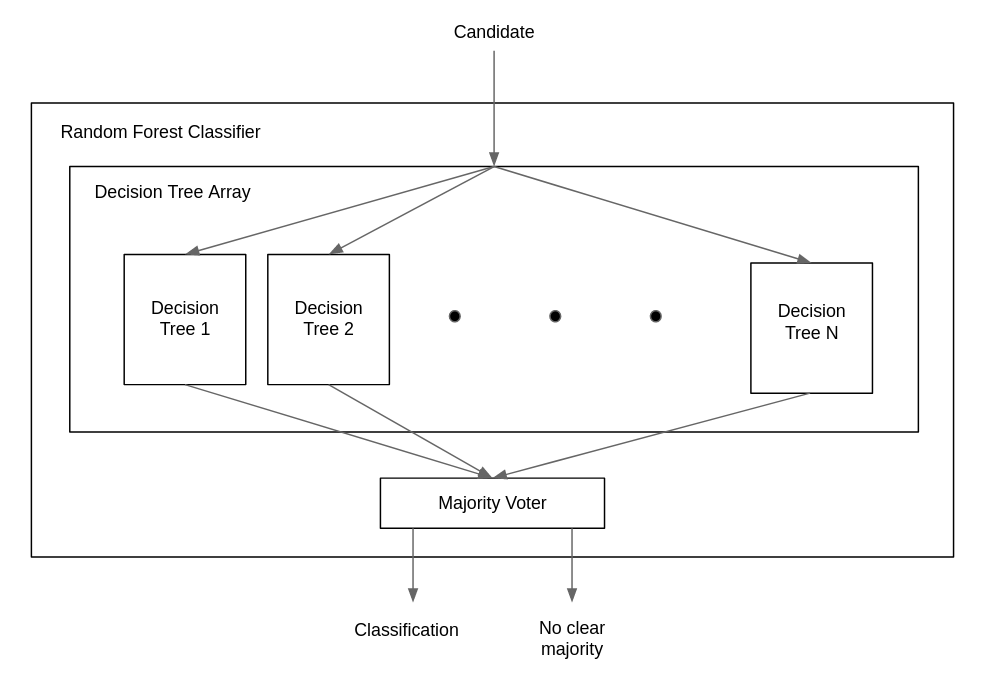
\includegraphics[width=250pt]{../images/architecture.png}
\end{center}
\end{frame}

\begin{frame}[label={sec:orgdf07850}]{Decision tree module}
This module stores a decision tree in an internal ROM and performs tree traversal when a candidate arrives for testing.
\end{frame}

\begin{frame}[label={sec:orgd8cf70d}]{Flowchart of the decision tree module}
\begin{center}
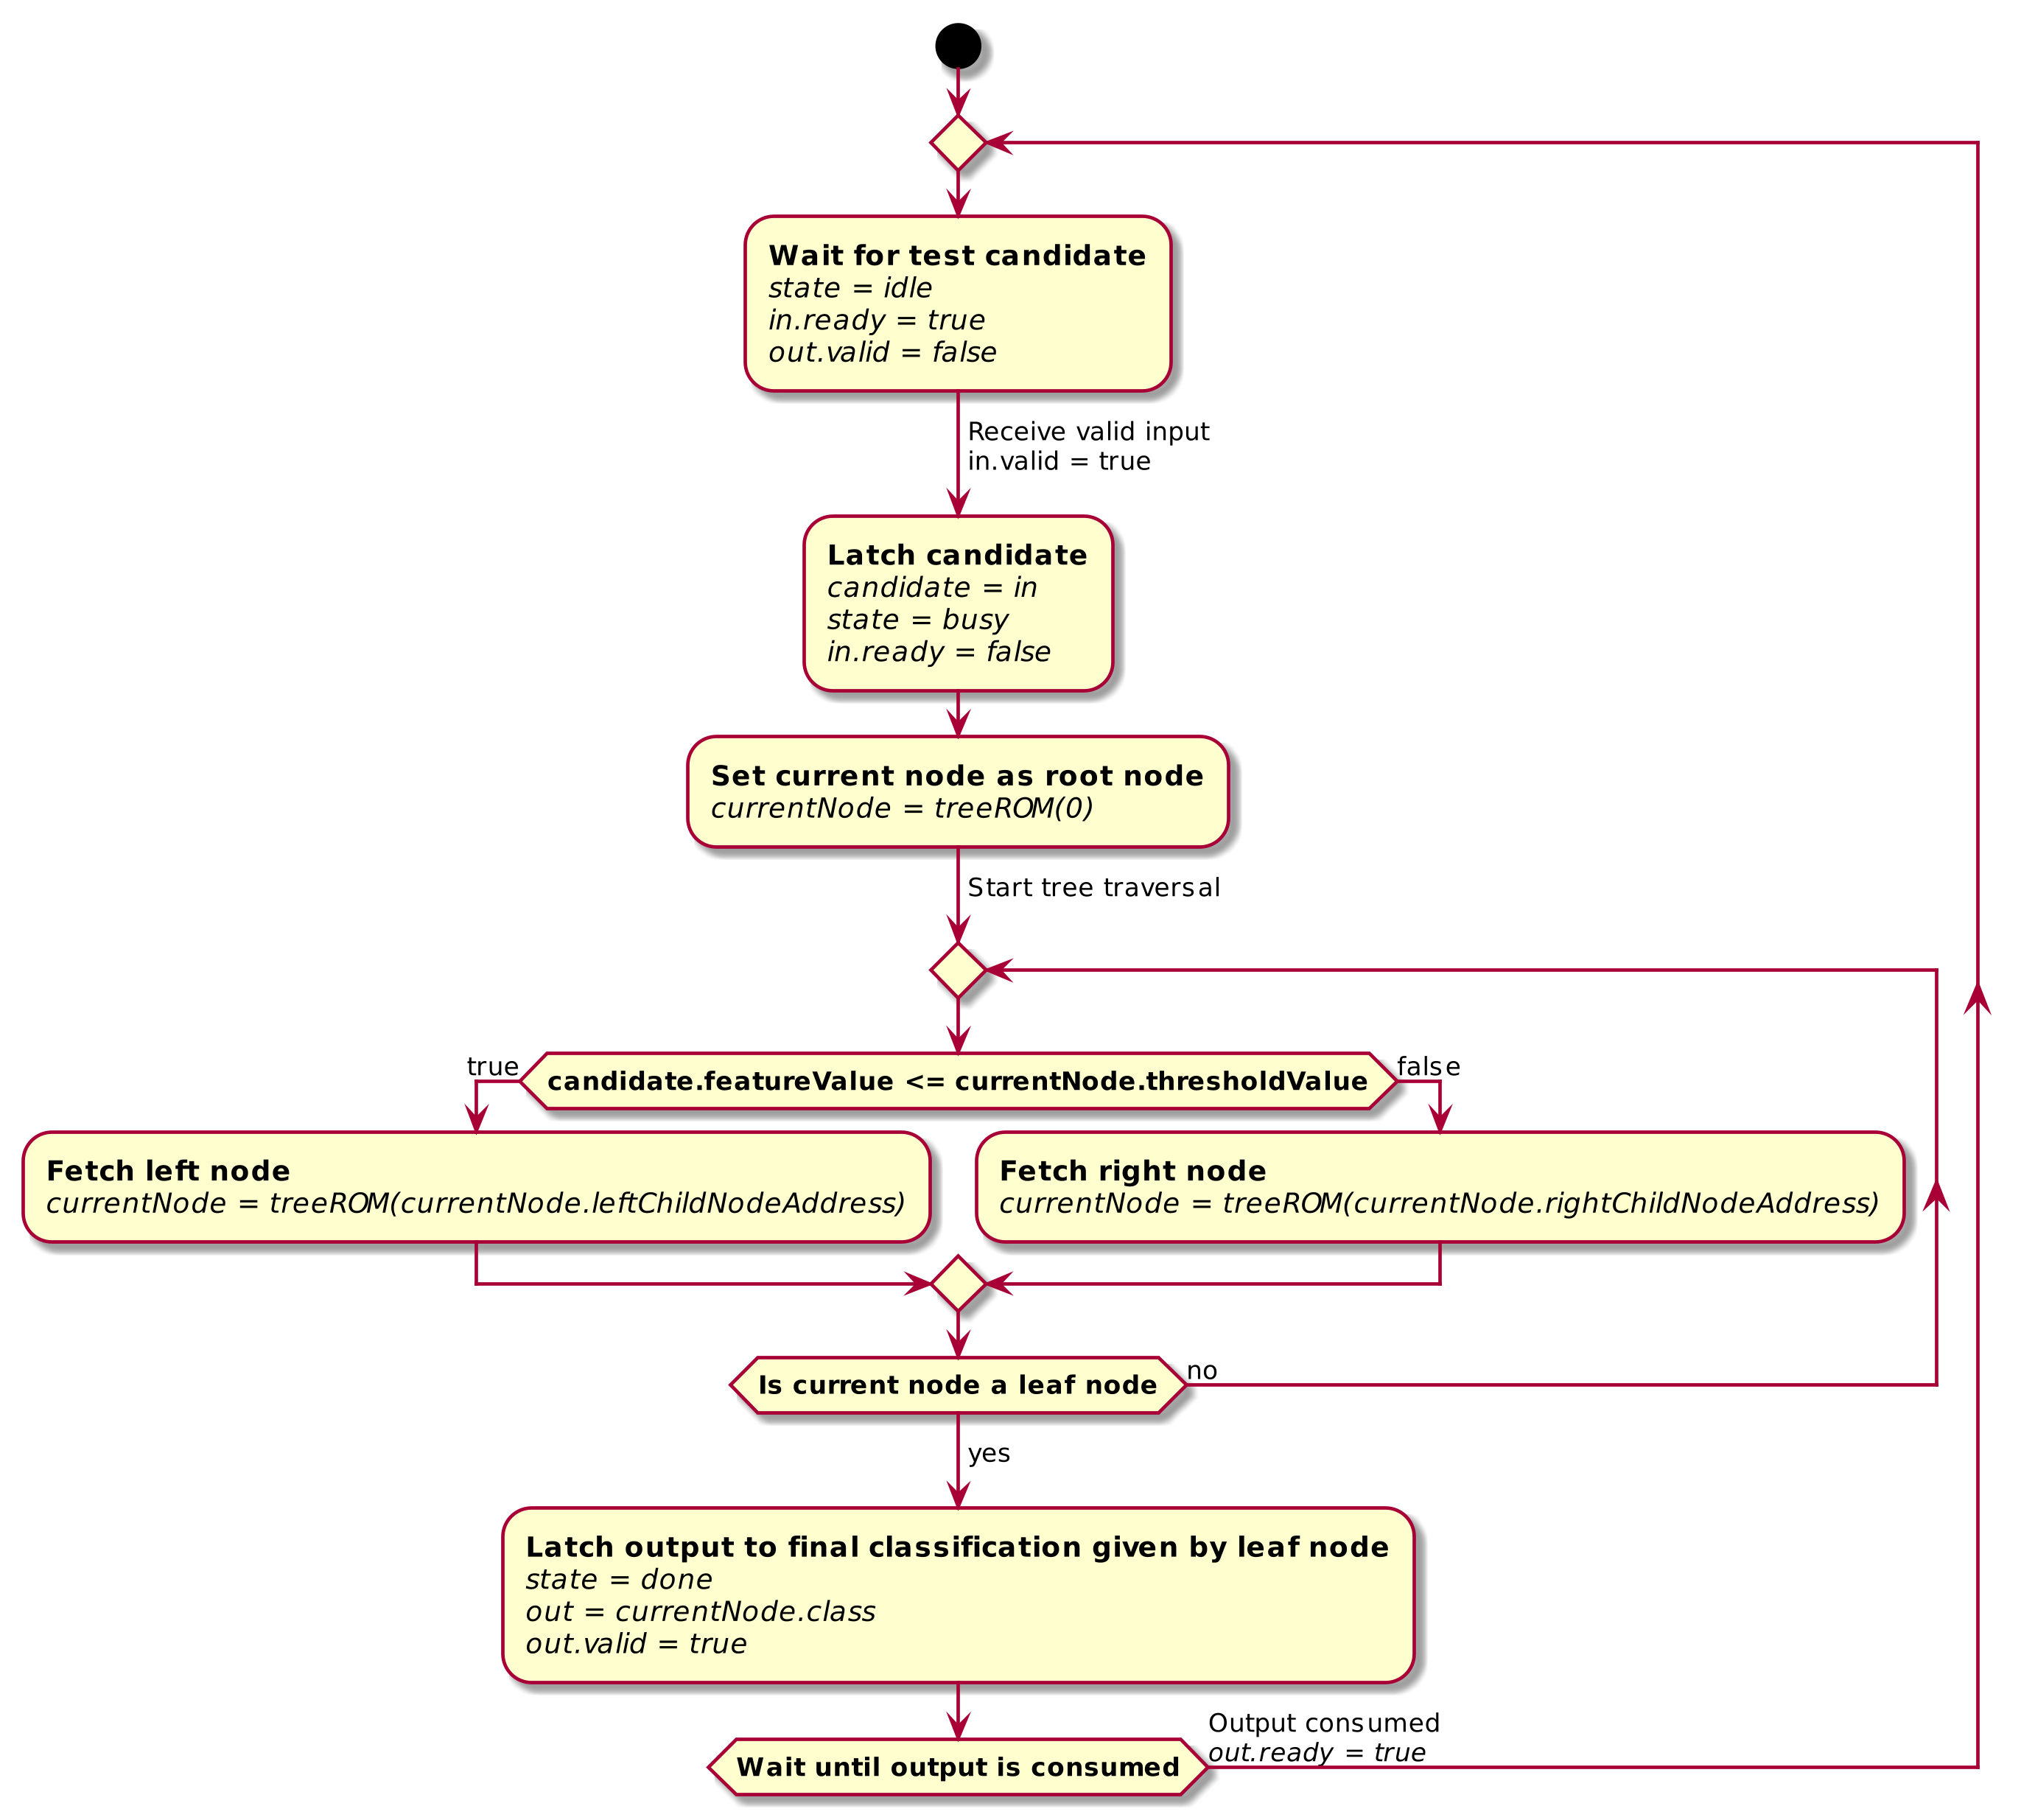
\includegraphics[width=250pt]{../schematics/DecisionTree/flow.png}
\end{center}
\end{frame}

\begin{frame}[label={sec:orgfe217d2}]{Structure of a node in the decision tree ROM}
\begin{center}
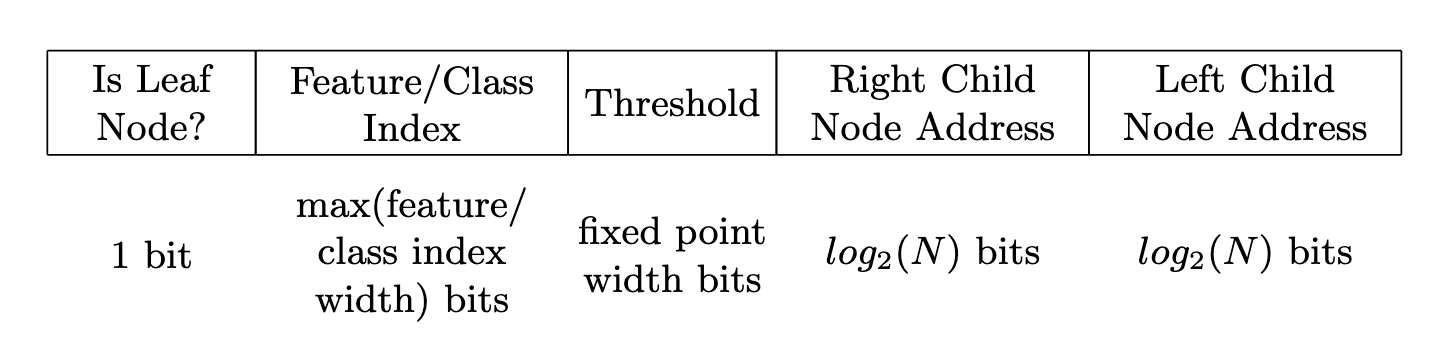
\includegraphics[width=.9\linewidth]{../schematics/DecisionTree/node-structure.png}
\end{center}
\end{frame}

\begin{frame}[label={sec:org9ff0b97}]{Decision tree array module}
This module consists of multiple decision tree modules that form the random forest. It handles the passing of test candidates to the various trees.
\end{frame}

\begin{frame}[label={sec:orge08c183}]{Majority voter module}
This modules takes as inputs form the individual trees and makes the final decision regarding the classification of the data point.
\begin{itemize}
\item The class getting the maximum votes (from each of the decision trees) is declared as the final class of the test candidate.
\item In case a majority is not achieved (two or more classes getting same number of votes) a separate ”no clear majority” flag is asserted.
\end{itemize}
\end{frame}

\begin{frame}[label={sec:org9ff3c29}]{Random Forest Classifier module}
This modules ties the decision tree array module to the majority voter module. The input to this module are the test candidates and the output are their corresponding classes.
\end{frame}

\begin{frame}[label={sec:org43efdb2}]{Run stage}
The run stage takes the generated verilog and performs the necessary actions based on the build target. It either builds and runs the verilator-based simulator or outputs the generated verilog file for further syntheis with external FPGA toolchains.
\end{frame}
\section*{Observations, features and conclusions}
\label{sec:org57aaff2}
\begin{frame}[label={sec:orga304214}]{Observations}
The project was tested with the HTRU 2 dataset and some key observations were made. These are presented in the following slides
\end{frame}
\begin{frame}[label={sec:org9d1c1fc}]{Discrepancy between software and hardware majority voting}
It was noted that there are a relatively small number of discrepancies between the hardware and software predictions. This is because software prediction algorithms uses a confidence based system for finding the final classification while hardware uses a voting based system. \emph{This has even lead to cases where hardware gives correct prediction relative to the target while the software is wrong.}

\begin{exampleblock}{Pros}
\begin{itemize}
\item Prediction method in hardware is much simpler as it uses integer comparisons as opposed to floating point based operations in software.
\end{itemize}
\end{exampleblock}

\begin{alertblock}{Cons}
\begin{itemize}
\item Hardware has higher chance of encountering ``No Clear Majority'' cases than software.
\end{itemize}
\end{alertblock}
\end{frame}

\begin{frame}[label={sec:orgb31b19f}]{Decision trees and other configurations being baked into hardware design}
It can be observed that the generated design is not generic and the RFC model is baked into it.

\begin{exampleblock}{Pros:}
\begin{itemize}
\item The hardware architecture is leaner as it does not need to deal with memory arbitration or external communication for acquiring the decision trees.
\end{itemize}
\end{exampleblock}

\begin{alertblock}{Cons:}
\begin{itemize}
\item If any changes are to be made to the model it would require the design to be recompiled from chisel, resynthesised and loaded on to the FPGA. This is unfavorable for cases where online learning may be required.
\end{itemize}
\end{alertblock}
\end{frame}

\begin{frame}[label={sec:org30ac9cf}]{Salient features}
Some salient features of the implementation:
\begin{itemize}
\item Input JSON configuration make the project more versatile and user-friendly
\item Implementation of circuits using highly parameterized chisel generators make the design highly scalable (any number of decision trees of any size)
\item Supports trees of varying depth
\item Simpler implementation as the ROMs are baked into the design
\item Automatic code generative architecture
\end{itemize}
\end{frame}

\begin{frame}[label={sec:org90f65fa}]{Project documentation}
\begin{itemize}
\item Paper can serve as primary documentation.
\item Developer oriented documentation on build system and configuration system have been added to the codebase.
\item The code has also been documented with scaladoc and comments.
\end{itemize}
\end{frame}

\begin{frame}[label={sec:orgde48054}]{}
\centering
\usebeamerfont*{frametitle}
\usebeamercolor[fg]{frametitle}
Thank you!
\end{frame}
\end{document}
